\begin{surferPage}[Kummer-Quartik]{Die Kummer-Quartik}
  Eduard Kummer war 1875 der erste, der explizit die Frage nach der maximalen Anzahl, genannt $\mu(d)$, von Singularitäten auf einer Fläche vom Grad d formulierte, und zwar für Flächen vom Grad 4, d. h. {\it  Quartiken}.\\
Er zeigte, dass $\mu(4) = 16$ ist und untersuchte in der Folgezeit Flächen mit dieser Eigenschaft im Detail. Eine besonders schöne Familie solcher Flächen ist gegeben durch:
\[
\bigl(x^2+y^2+z^2-\mu^2\bigr)^2-\lambda y_0 y_1 y_2 y_3,
\]
wobei $\mu$ ein frei wählbarer Parameter ist  und $\lambda$ von $\mu$ abhängt. Die $y_i$ sind, damit die Fläche symmetrisch ist, als die Seiten eines regelmäßigen Tetraeders  {\small
    $y_0=1-z-\sqrt{2}x$, \  
    $y_1=1-z+\sqrt{2}x$, \ 
    $y_2=1+z+\sqrt{2}y$, \ 
    $y_3=1+z-\sqrt{2}y$} gewählt. \\
Nicht alle Mitglieder dieser Familie haben genau 16 reelle Singularitäten, die meisten aber schon. 
\newline

 \begin{center}
      \vspace{-0.2cm}
      \begin{tabular}{@{}c@{\ }c@{\ }c@{\ }c@{}}
        \begin{tabular}{@{}c@{}}
          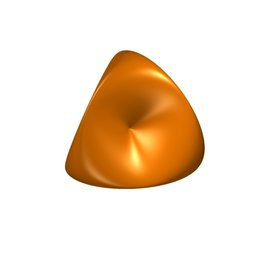
\includegraphics[width=1.35cm]{./../../common/images/kummer_0}
        \end{tabular}
        &
        \begin{tabular}{@{}c@{}}
          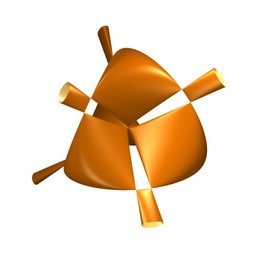
\includegraphics[width=1.35cm]{./../../common/images/kummer_1}
        \end{tabular}
        &
        \begin{tabular}{@{}c@{}}
          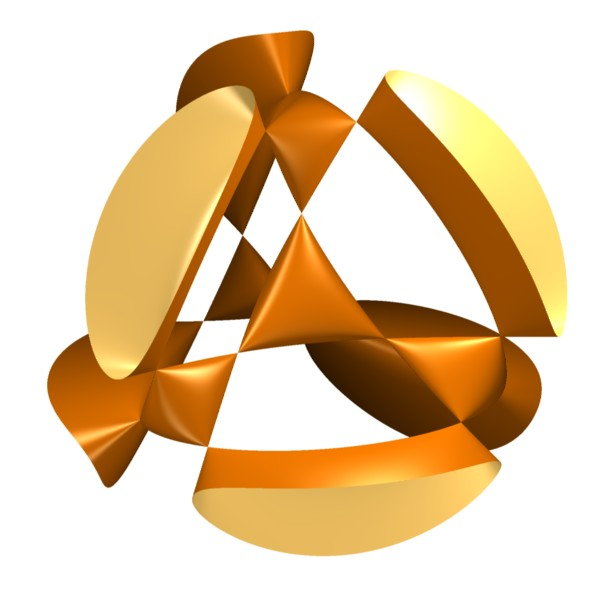
\includegraphics[width=1.35cm]{./../../common/images/kummer_2}
        \end{tabular}
        &
        \begin{tabular}{@{}c@{}}
          
\includegraphics[width=1.35cm]{./../../common/images/kummer_3}
        \end{tabular}
      \end{tabular}
    \end{center}
      \vspace{-0.2cm}  
  F\"ur spezielle Werte der Parameter k\"onnen mehrere Singularit\"aten aufeinander fallen.
\end{surferPage}
